%==============================================================================
% Sjabloon onderzoeksvoorstel bachelorproef
%==============================================================================
% Gebaseerd op LaTeX-sjabloon ‘Stylish Article’ (zie voorstel.cls)
% Auteur: Jens Buysse, Bert Van Vreckem
%
% Compileren in TeXstudio:
%
% - Zorg dat Biber de bibliografie compileert (en niet Biblatex)
%   Options > Configure > Build > Default Bibliography Tool: "txs:///biber"
% - F5 om te compileren en het resultaat te bekijken.
% - Als de bibliografie niet zichtbaar is, probeer dan F5 - F8 - F5
%   Met F8 compileer je de bibliografie apart.
%
% Als je JabRef gebruikt voor het bijhouden van de bibliografie, zorg dan
% dat je in ``biblatex''-modus opslaat: File > Switch to BibLaTeX mode.

\documentclass{voorstel}
\usepackage{graphicx}
\usepackage{lipsum}


%------------------------------------------------------------------------------
% Metadata over het voorstel
%------------------------------------------------------------------------------

%---------- Titel & auteur ----------------------------------------------------

% TODO: geef werktitel van je eigen voorstel op
\PaperTitle{Invloed van ongunstige omstandigheden op low-cost GPS tracking devices: Onderzoek en proof of concept}
\PaperType{Onderzoeksvoorstel Bachelorproef 2019-2020} % Type document

% TODO: vul je eigen naam in als auteur, geef ook je emailadres mee!
\Authors{Indy Van Canegem\textsuperscript{1}} % Authors
\CoPromotor{Jens Buysse\textsuperscript{2} (Hogeschool Gent)}
\affiliation{\textbf{Contact:}
  \textsuperscript{1} \href{mailto:Indy.vancanegem@student.hogent.be}{Jens.buysse@student.hogent.be};
  \textsuperscript{2} \href{mailto:Indy.vancanegem4@student.hogent.be}{Jens.buysse@student.hogent.be};
}

%---------- Abstract ----------------------------------------------------------

\Abstract{In deze bachelorproef wordt er onderzocht wat de kwaliteit bepaalt van een GPS-systeem. Naast het bepalen van je huidige locatie, kunnen ze ook gebruikt worden binnen water- en wintersporten. Zo kan tijdens het surfen plots het surfbord wegdrijven, wat veel geld kan kosten. Een andere toepassing is dat men tijdens het snowboarden lawineslachtoffers kan lokaliseren met behulp van een lawinepieper. Aan de hand van een proof of concept wordt er onderzoek gedaan naar de verschillen van GPS-systemen en wordt er duidelijkheid geschept over hoe GPS-systemen kwalitatief blijven werken in ongunstige omstandigheden zoals water en sneeuw. De proof of concept dient naast kwalitatief, ook low-cost te zijn zodat het toegankelijker is naar water- en wintersporters toe. 
}

%---------- Onderzoeksdomein en sleutelwoorden --------------------------------
% TODO: Sleutelwoorden:
%
% Het eerste sleutelwoord beschrijft het onderzoeksdomein. Je kan kiezen uit
% deze lijst:
%
% - Mobiele applicatieontwikkeling
% - Webapplicatieontwikkeling
% - Applicatieontwikkeling (andere)
% - Systeembeheer
% - Netwerkbeheer
% - Mainframe
% - E-business
% - Databanken en big data
% - Machineleertechnieken en kunstmatige intelligentie
% - Andere (specifieer)
%
% De andere sleutelwoorden zijn vrij te kiezen

\Keywords{Onderzoeksdomein. GPS – AGPS – Raspberry Pi – SPS – PPS – gsm} % Keywords
\newcommand{\keywordname}{Sleutelwoorden} % Defines the keywords heading name

%---------- Titel, inhoud -----------------------------------------------------

\begin{document}

\flushbottom % Makes all text pages the same height
\maketitle % Print the title and abstract box
\tableofcontents % Print the contents section
\thispagestyle{empty} % Removes page numbering from the first page

%------------------------------------------------------------------------------
% Hoofdtekst
%------------------------------------------------------------------------------

% De hoofdtekst van het voorstel zit in een apart bestand, zodat het makkelijk
% kan opgenomen worden in de bijlagen van de bachelorproef zelf.
%---------- Inleiding ---------------------------------------------------------

\section{Introductie} % The \section*{} command stops section numbering
\label{sec:introductie}

Een van de meest verspreide ICT-toepassingen als gevolg van de recente technologische revolutie is het Global Positioning System (GPS). Met GPS wordt er impliciet verwezen naar de Standard Positioning Service (SPS). De SPS is een positionerings- en timingdienst die wordt aangeboden door middel van variërende signalen die worden uitgezonden op de GPS L1 frequentie \autocite{gps_def}.  Deze technologische toepassing heeft verregaande gevolgen gehad inzake de manier waarop onze samenleving georganiseerd wordt. Mensen gebruiken de GPS om files te ontwijken op weg naar hun werk en om niet te verdwalen op reis, maar GPS systemen kunnen ook  gebruikt worden voor water- en wintersporten. Praktische voorbeelden hiervan zijn lawinepiepers. Een lawinepieper is een radiozender en -ontvanger die wordt gebruikt om mensen op te sporen die onder een lawine zijn geraakt \autocite{avalanche_performance}. 

Lawinepiepers zijn vaak niet goedkoop en er bestaan weinig goedkope alternatieven die dezelfde kwaliteit behouden. Lawinepiepers zijn te verkrijgen vanaf ongeveer 200 euro. Tussen de verschillende merken van deze lawinepiepers heerst er een groot verschil aan kwaliteit en prijs. In deze bachelorproef wordt er nagegaan of het mogelijk is om een product te ontwikkelen dat even kwalitatief werkt als professionele toestellen die momenteel gebruikt kunnen worden in ongunstige omstandigheden zoals bij het uitoefenen van water- en wintersporten, maar dan goedkoper.


%---------- Stand van zaken ---------------------------------------------------

\section{State-of-the-art}
\label{sec:state-of-the-art}

Volgens \textcite{avalanche_performance} is het niet vanzelfsprekend om iemand te vinden met behulp van lawinepiepers. Het vinden van de beacon hangt sterk af van welk merk er gebruikt wordt. Uit het onderzoek van \textcite{avalanche_performance} blijkt dat er een significant verschil is in de kwaliteit van de toestellen en in de tijd waarin het duurt om iemand terug te vinden. Het tijdsbestek waarin fictieve lawineslachtoffers teruggevonden werden, varieert tussen 109,5 seconden en 215 seconden. In beide gevallen werd de mediaan gebruikt voor het bepalen van het tijdsbestek per model.
De kwaliteit van deze toestellen kan afhangen van welke GPS-service ze gebruik maken. Zo is er de Standard Positioning Service (SPS), die als minder nauwkeurig beschouwd wordt, en de Precise Positioning Service (PPS). De SPS-service is vrij te gebruiken door particulieren en bedrijven, terwijl de PPS-service een autorisatie vereist die in de praktijk alleen te gebruiken valt voor militaire toepassingen. \autocite{gps_performances} Lawinepiepers zijn niet geautoriseerd om PPS te kunnen gebruiken, waardoor we deze GPS-service level uitsluiten in dit onderzoek. 
Naast de twee GPS-service levels (SPS en PPS) bestaan er ook alternatieve manieren om locaties te bepalen. We hebben het traditionele Global Positioning System (GPS), dat gebruikt maakt van satellieten, maar ook Assisted Global Positioning Systems (A-GPS), die daarnaast ook gebruik maakt van masten voor mobiele telefoons. \autocite{a_gps_vs_gps} Een andere mogelijkheid is het gebruik van De Flemish Positioning Service.
In deze bachelorproef wordt er een proof of concept (PoC) opgeleverd die gebruik zal maken van de besproken technologieën. Deze PoC zal bestaan uit een Rasberry Pi 3 (RP3), aangezien deze voldoet aan de volgende vereisten: low-cost, mogelijkheid tot gebruik van GPS en mogelijkheid tot waterdichte casing. Voor waterdichtheid en bescherming van de RP3 zal er gebruik gemaakt worden van een plastic omhulsel,  aangezien deze meer resistent zijn in ongunstige omstandigheden dan metaal \autocite{plastic_corrosion}.
Bij dit onderzoek kan de volgende hypothese opgesteld worden en proberen we de nulhypothese te verwerpen:
H1: Het is mogelijk om een low-cost GPS-systeem te ontwikkelen die bijna even kwalitatief is als een bestaand professioneel toestel die overleeft in ongunstige omstandigheden (water/sneeuw/zout).
H0: Het is niet mogelijk om een low-cost GPS-systeem te ontwikkelen die een gelijkaardige kwaliteit bevat als een bestaand professioneel toestel dat overleeft in ongunstige omstandigheden (water/sneeuw/zout).

%---------- Methodologie ------------------------------------------------------
\section{Methodologie}
\label{sec:methodologie}

Er zullen experimenten/simulaties uitgevoerd worden waarbij de PoC gemonitord en vergeleken wordt met reeds bestaande toestellen. Hiervoor zullen er field tests uitgevoerd worden.  Na de field tests wordt er bekeken hoe de PoC verbeterd kan worden om de kwaliteit van de reeds bestaande toestellen te evenaren en tegelijkertijd een low-cost device te blijven. 
Zo willen we de maximale diepte bepalen waarop de PoC een GPS-signaal blijft sturen, en dit zowel in water als in sneeuw. Ook de mate waarin de locatiebepaling accuraat is, wordt onder de loep genomen. 
Volgens \autocite{gps_water} zouden GPS-signalen zich niet goed kunnen verplaatsen in water. Vreemd genoeg claimt het merk divenetgps een diepte te bereiken van 300m. Voor de wetenschappelijke relevantie wordt getest hoe diep een GPS-systeem blijft functioneren naar behoren onder water. Indien dit mogelijk is, kunnen er toepassingen uitgewerkt worden binnen watersporten, zoals het terugvinden van een surfboard.
Om uit te schijnen tussen bestaande toestellen zal de gebruiksvriendelijkheid ook verbetert worden door middel van een applicatie die het ‘tracken’ van iets of iemand zeer eenvoudig maakt.


%---------- Verwachte resultaten ----------------------------------------------

\section{Verwachte resultaten}
\label{sec:verwachte_resultaten}
Voor de volgende grafieken geldt: (Deze grafieken zijn fictief, ze zijn slechts een verwachting)
\newline
PD = Professional Device, bestaand product op de markt
\newline
PoC = zelf ontwikkelde Proof of Concept
\clearpage
Verwachte resultaten van field tests in ongunstige omstandigheden (sneeuw):
\newline
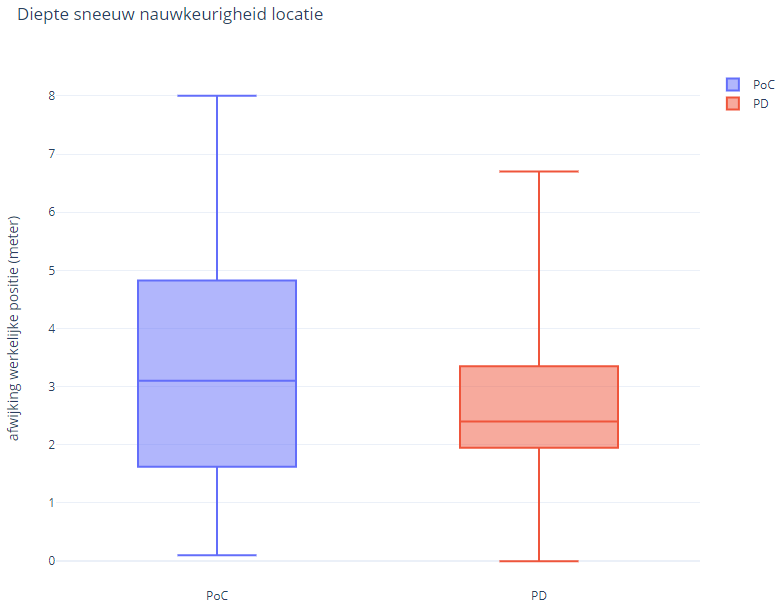
\includegraphics[width=\textwidth,height=\textheight,keepaspectratio]{snowAccuracy}
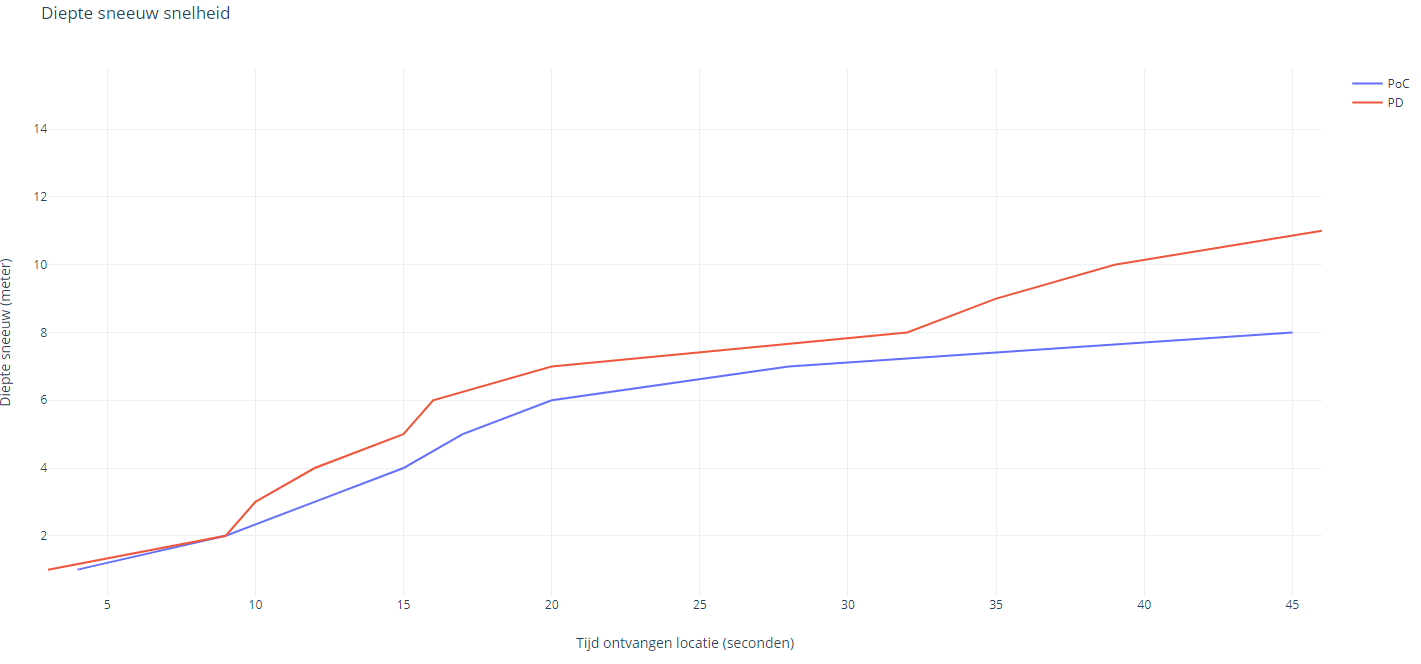
\includegraphics[width=\textwidth,height=\textheight,keepaspectratio]{snowDepth}
\clearpage
Verwachte resultaten van field tests in ongunstige omstandigheden (water):
\newline
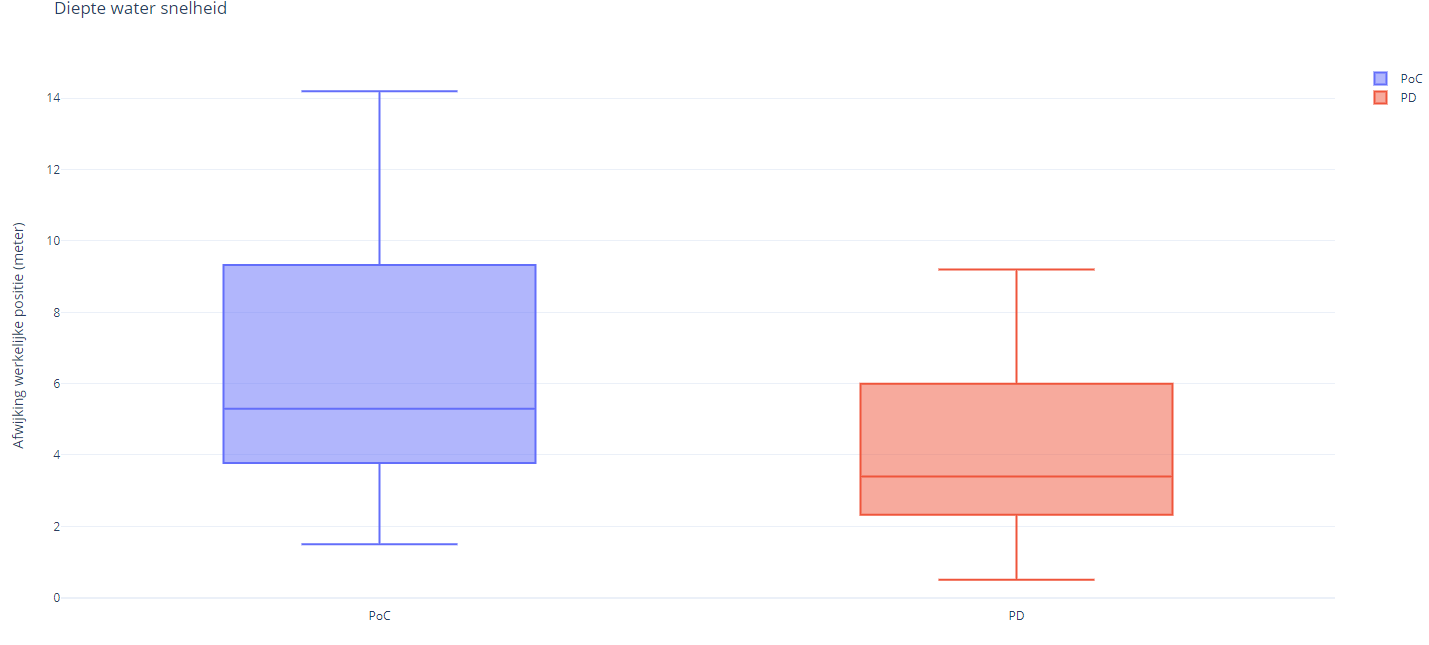
\includegraphics[width=\textwidth,height=\textheight,keepaspectratio]{waterAccuracy}
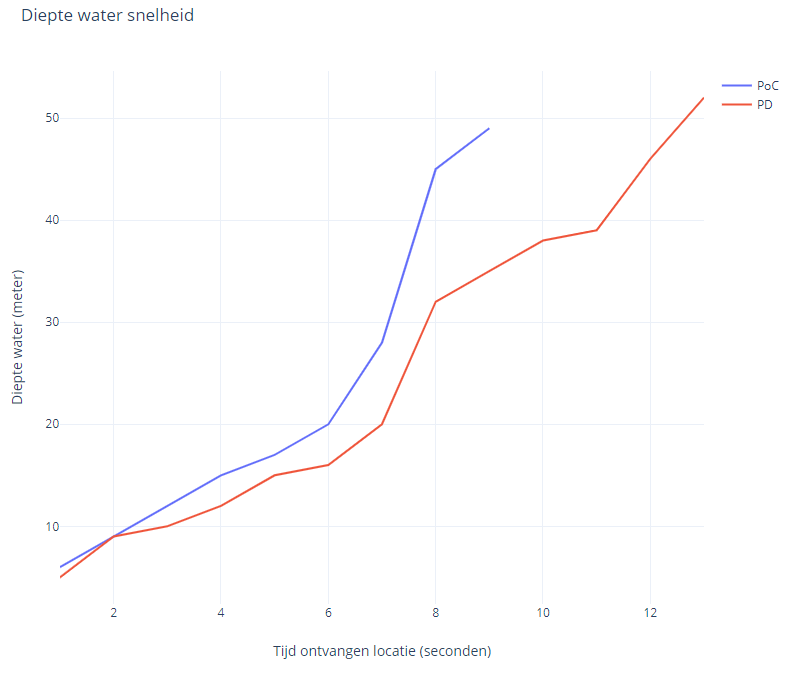
\includegraphics[width=\textwidth,height=\textheight,keepaspectratio]{waterDepth}
\clearpage
%---------- Verwachte conclusies ----------------------------------------------
\section{Verwachte conclusies}
\label{sec:verwachte_conclusies}

Uit dit onderzoek moet duidelijk blijken of het mogelijk is een low-cost GPS-systeem te ontwikkelen dat niet onderdoet voor de bestaande producten. De PoC zal relatief goede resultaten behalen ten opzichte van de producten die al op de markt zijn. 
Hopelijk vloeit uit dit onderzoek een PoC voort die klaar is voor de consument die opzoek is naar een GPS-systeem van vergelijkbare kwaliteit die gebruikt kan worden voor doeleinden zoals het vinden van een verloren surfboard tot het terugvinden van lawineslachtoffers.




%------------------------------------------------------------------------------
% Referentielijst
%------------------------------------------------------------------------------
% TODO: de gerefereerde werken moeten in BibTeX-bestand ``voorstel.bib''
% voorkomen. Gebruik JabRef om je bibliografie bij te houden en vergeet niet
% om compatibiliteit met Biber/BibLaTeX aan te zetten (File > Switch to
% BibLaTeX mode)

\phantomsection
\printbibliography[heading=bibintoc]

\end{document}
